\section*{Swapping (transparent to process)}
\begin{itemize}
\item For more than avail. physical memory $\to$ use 2nd storage, SSD etc.
\item Space on disk reserved to move pages back/forth to memory
\item OS reads/writes to swap space in \textbf{page-sized} units
\item OS needs to remember disk address of a given page
\item TLB uses this bit to track if a page is present in physical memory
\end{itemize}
\section*{Why hardware doesn't handle page faults}
\begin{enumerate}
\item page faults to disk are \emph{slow}; extra overheads of software are minimal
\item the hardware would have to understand swap space, how to issue I/Os to disk, and lots other details it currently doesn't know much about
\end{enumerate}
\section*{OS handles page faults via swapping}
while I/O is in flight, process will be in blocked state. Thus, OS will be free to run other ready processes while page fault is being serviced
\begin{enumerate}
\item page tables stores bits info about where to find the desired page
\item OS uses the bits in PTE for a disk address
\item On page fault, OS looks in PTE to find the address and issues request to disk to fetch page into memory
\item When disk I/O done, OS marks the page in PT as present, update PFN field of PTE to record in-memory location of newly-fetched page, and retry ix
\item This next attempt may cause TLB miss which would then be serviced and update TLB with addr translation (or update TLB directly)
\item a last restart would find the translation in TLB and proceed to fetch desired data/instruction from memory at translated physical address
\end{enumerate}
\section*{Page-Fault Control Flow Algorithm (Hardware)}
\begin{minipage}{.72\linewidth}
\begin{lstlisting}[language=c]
VPN = (VirtualAddress & VPN_MASK) >> SHIFT
(Success, TlbEntry) = TLB_Lookup(VPN)
if (Success == True) // TLB Hit
   if (CanAccess(TlbEntry.ProtectBits) == True)
      Offset = VirtualAddress & OFFSET_MASK
      PhysAddr = (TlbEntry.PFN << SHIFT) | Offset
      Register = AccessMemory(PhysAddr)
   else
      RaiseException(PROTECTION_FAULT)
else                 // TLB Miss
   PTEAddr = PTBR + (VPN * sizeof(PTE))
   PTE = AccessMemory(PTEAddr)
   if (PTE.Valid == False)
      RaiseException(SEGMENTATION_FAULT)
   else
      if (CanAccess(PTE.ProtectBits) == False)
         RaiseException(PROTECTION_FAULT)
      else if (PTE.Present == True)
         // assuming hardware-managed TLB
         TLB_Insert(VPN, PTE.PFN, PTE.ProtectBits)
         RetryInstruction()
      else if (PTE.Present == False)
         RaiseException(PAGE_FAULT)
\end{lstlisting}
\end{minipage}
\begin{minipage}{.28\linewidth}
  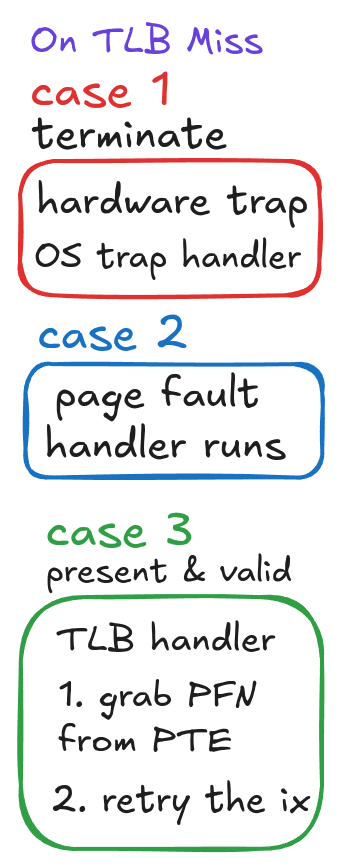
\includegraphics[width=\linewidth]{imgs/swap_cases}
\end{minipage}
\section*{Page-Fault Control Flow Algorithm (Software)}
\begin{minipage}{.72\linewidth}
\begin{lstlisting}[language=c]
PFN = FindFreePhysicalPage()
if (PFN == -1)                 // no free page found
    PFN = EvictPage()          // replacement algo
DiskRead(PTE.DiskAddr, PFN)  // sleep (wait for I/O)
PTE.present = True             // update page table:
PTE.PFN = PFN                  // present/translation
RetryInstruction()             // retry instruction
\end{lstlisting}
\end{minipage}
\begin{minipage}{.28\linewidth}
  \flushleft
  \begin{enumerate}
  \item check any free pages avail
  \item if not, ask bg thread to free
  \item when some pages avail, wake up orig thread
  \end{enumerate}
\end{minipage}

\begin{itemize}
\item when OS notices there're fewer than low watermark (LW) pages avail., a background thread responsible for freeing memory runs
\item bg thread evicts pages until there're high watermark (HW) pages avail.
\item bg swap/page daemon: disk efficiency $\uparrow$; work $\downarrow$, better idle time
\item OS groups pages and swaps them out at once $\to$ $\uparrow$ disk efficiency
\end{itemize}
